\documentclass[a4paper]{article}

% Language and font encodings
\usepackage[english]{babel}
\usepackage[utf8x]{inputenc}
\usepackage[T1]{fontenc}
\usepackage[a4paper,top=3cm,bottom=2cm,left=3cm,right=3cm,marginparwidth=1.75cm]{geometry}
\usepackage{titling}
\usepackage{amsmath}
\usepackage{titlesec}
\usepackage{graphicx}
\usepackage{tabularx}
\usepackage[colorinlistoftodos]{todonotes}
\usepackage[colorlinks=true, allcolors=blue]{hyperref}
\usepackage{fancyhdr}
\usepackage{wrapfig}
\usepackage{subcaption}

\graphicspath{{images/}}

\title{Cosmology Assignment 1}
\author{Daniel Herman: daniel.herman@astro.uio.no}

\begin{document}

\begin{titlepage}
\maketitle
\end{titlepage}

\textbf{Exercise 1.}

\noindent (1) Show that in a universe that is undergoing Hubble expansion, that $\bar{\rho}(t)=\bar{\rho}(t=t_0)a^{-3}$, where $t_0$ denotes the age of the Universe today:\\

We use the definition $\vec{v_r} = H \vec{r_r}$, and the continuity equation $\dfrac{d\rho_0}{dt} + \rho_0 \nabla \cdot \vec{v_0}.$\\

So, $\dfrac{d\rho_0}{dt} + 3\rho_0 \dfrac{\dot{a}}{a} = 0 \Rightarrow \dfrac{d\rho_0}{dt} = -3\rho_0 \dfrac{\dot{a}}{a}$. Now we integrate both sides.\\
$$\int \dfrac{\dot{\rho_0}}{\rho_0} = -3 \int \dfrac{\dot{a}}{a} \Rightarrow \ln \dfrac{\bar{\rho}}{\rho} = -3 \ln a \Rightarrow \dfrac{\bar{\rho}}{\rho} = a^{-3} \Rightarrow \bar{\rho} = \rho a^{-3} $$.\\

\noindent (2) Derive the perturbed Poisson's and Euler's Equations.\\
Poisson's Equation: $$ \nabla^2(\phi_0 + \delta\phi) = 4 \pi G(\rho_0 + \delta\rho) \Rightarrow \nabla^2\phi_0 + \nabla^2\delta\phi = 4 \pi G \rho_0 + 4 \pi G \delta \rho$$.\\ Since $\nabla^2\phi_0 = 4 \pi G \rho_0,$ 
\begin{equation}
\nabla^2\delta\phi = 4 \pi G \delta \rho
\label{eq:1}
\end{equation}

\noindent Euler's Equation: $ \dfrac{dv_0}{dt} = -\dfrac{1}{\rho_0} \nabla p_0 - \nabla \phi_0$. We need to break apart this problem to successfully derive the solution.\\
We utilize the definition of the time derivative for comoving space: $\dfrac{d}{dt} = (\dfrac{\partial}{\partial t} + \vec{v}\cdot \nabla)$.\\
\noindent We defined the perturbed quantities as follows:\\ Pressure: $p = p_0 + \delta p.$ \\
Velocity: $\vec{v} = \vec{v_0} + \delta\vec{v}$\\
Potential: $\nabla \phi = \nabla (\phi_0 + \delta \phi) = \nabla \phi_0 + \nabla \delta \phi$\\ 
Density: $\dfrac{1}{\rho} = \dfrac{1}{\rho_0 + \delta \rho}$\\ 
And we rewrite the unperturbed Euler's equation below:
\begin{equation}
\dfrac{d\vec{v_0}}{dt} = (\dfrac{\partial}{\partial t} + \vec{v_0} \cdot \nabla) \vec{v_0} = \dfrac{\partial \vec{v_0}}{\partial t} + (\vec{v_0} \cdot \nabla) \vec{v_0}  = -\dfrac{1}{\rho_0} \nabla p_0 - \nabla \phi_0
\label{eq:2}
\end{equation}

\noindent First we will derive the L.H.S.:\\

\begin{center}
$\dfrac{d\vec{v}}{dt} = \dfrac{d(\vec{v_0}+\delta \vec{v})}{dt} = \dfrac{\partial}{\partial t}(\vec{v_0} + \delta \vec{v}) + (\vec{v_0}+\delta \vec{v}) \cdot \nabla (\vec{v_0}+\delta \vec{v})$
\end{center}

\begin{equation}
= \dfrac{\partial \vec{v_0}}{\partial t} + \dfrac{\partial \delta \vec{v}}{\partial t} + (\vec{v_0} \cdot \nabla) \vec{v_0} + (\vec{v_0} \cdot \nabla)\delta \vec{v} + (\delta \vec{v} \cdot \nabla)\vec{v_0} + (\delta \vec{v} \cdot \nabla)\delta \vec{v}.
\label{eq:3} 
\end{equation}
\noindent The $(\delta \vec{v} \cdot \nabla) \delta \vec{v}$ term is equal to zero since we are taking a linear perturbation, so equation 3 becomes:\\
\begin{equation}
\dfrac{\partial \vec{v_0}}{\partial t} + \dfrac{\partial \delta \vec{v}}{\partial t} + (\vec{v_0} \cdot \nabla) \vec{v_0} + (\vec{v_0} \cdot \nabla)\delta \vec{v} + (\delta \vec{v} \cdot \nabla)\vec{v_0}
\label{eq:4}
\end{equation}
\noindent Now the R.H.S.:\\

\begin{equation}
- \dfrac{\nabla(p_0 + \delta p)}{\rho_o + \delta \rho} = - \dfrac{(\rho_0-\delta \rho) \nabla(p_0 + \delta p)}{\rho_o^2 - \delta \rho^2} - \nabla \phi_0 - \nabla \delta \phi 
\label{eq:5}
\end{equation}
Again, since this is a linear perturbation, $\delta \rho^2 = 0$.

\begin{center}
$= -\dfrac{\rho_0 \nabla p_0 - \delta \rho \nabla p_0 - \delta \rho \nabla \delta p + \rho_0 \nabla \delta p}{\rho_0^2}  - \nabla \phi_0 - \nabla \delta \phi  = - \dfrac{\nabla p_0 + \nabla \delta p}{\rho_0} - \nabla \phi_0 - \nabla \delta \phi$
\end{center}
Since we exclude these terms: $(\delta \rho \nabla p_0 = \delta \rho \nabla \delta p = 0)$\\
The perturbed Euler equation becomes:
\begin{align*}
\dfrac{\partial \vec{v_0}}{\partial t} + \dfrac{\partial \delta \vec{v}}{\partial t} + (\vec{v_0} \cdot \nabla) \vec{v_0} + (\vec{v_0} \cdot \nabla)\delta \vec{v} + (\delta \vec{v} \cdot \nabla)\vec{v_0} =& - \dfrac{\nabla p_0}{\rho_0} - \dfrac{\nabla \delta p}{\rho_0} - \nabla \phi_0 - \nabla \delta \phi\\
\Rightarrow \dfrac{d \vec{v_0}}{dt} + \dfrac{\partial \delta \vec{v}}{\partial t} + (\vec{v_0} \cdot \nabla)\delta \vec{v} + (\delta \vec{v} \cdot \nabla)\vec{v_0} =& - \dfrac{\nabla p_0}{\rho_0} - \dfrac{\nabla \delta p}{\rho_0} - \nabla \phi_0 - \nabla \delta \phi
\end{align*}

\noindent And removing the unperturbed portion (2) it simplifies to:

\begin{equation}
\dfrac{\partial \delta \vec{v}}{\partial t} + (\vec{v_0} \cdot \nabla)\delta \vec{v} + (\delta \vec{v} \cdot \nabla)\vec{v_0} = - \dfrac{\nabla \delta p}{\rho_0} - \nabla \delta \phi
\end{equation}

\noindent Utilizing the definition of the time derivative again, $\dfrac{\partial \delta \vec{v}}{\partial t} + (\vec{v_0} \cdot \nabla)\delta \vec{v} = \dfrac{d \delta \vec{v}}{dt}$, so we finally reach our result:

\begin{equation}
\dfrac{d \delta \vec{v}}{dt} + (\delta \vec{v} \cdot \nabla)\vec{v_0} = - \dfrac{\nabla \delta p}{\rho_0} - \nabla \delta \phi
\end{equation}

\noindent \textbf{Exercise 2.} (Code included at \url{https://github.com/hermda02/myfirstcosmology}) \\
(1) $H^2 = \big( \dfrac{\dot{a}}{a} \big)^2 = H_0^2 \Big[\dfrac{\Omega_m}{a^3} + \dfrac{\Omega_r}{a^4}+\Omega_{\Lambda} \Big]$ and $\dfrac{\Omega_r}{a^4} \rightarrow 0.$\\
Let $(\Omega_m, \Omega_{\Lambda})$ = (1.0,0.0); $\dfrac{\dot{a}}{a} = H_0 \cdot a^{-3/2} = H$ \\
Let $(\Omega_m, \Omega_{\Lambda})$ = (0.3,0.7); $\dfrac{\dot{a}}{a} = H_0 \Big[\dfrac{0.3}{a^3} + 0.7 \Big]^{1/2} = H  $\\
Let $(\Omega_m, \Omega_{\Lambda})$ = (0.8,0.2); $\dfrac{\dot{a}}{a} = H_0 \Big[\dfrac{0.8}{a^3} + 0.2 \Big]^{1/2} = H $\\
\begin{figure}[h]
\centering
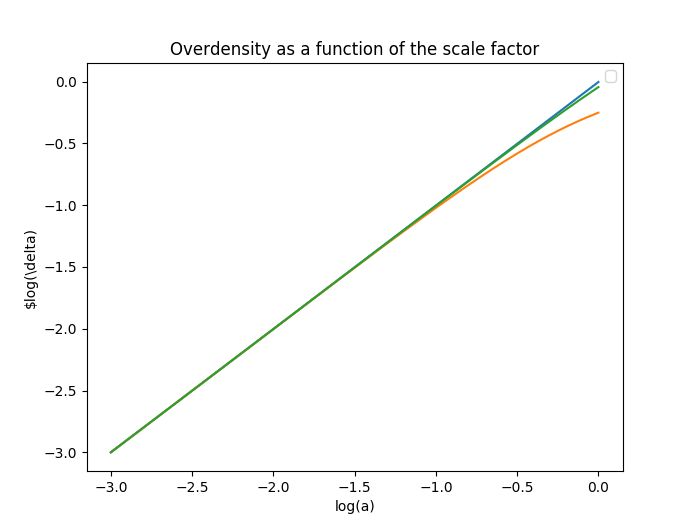
\includegraphics[scale=0.475]{exercise2-1}
\end{figure}
\begin{figure}[h]
\centering
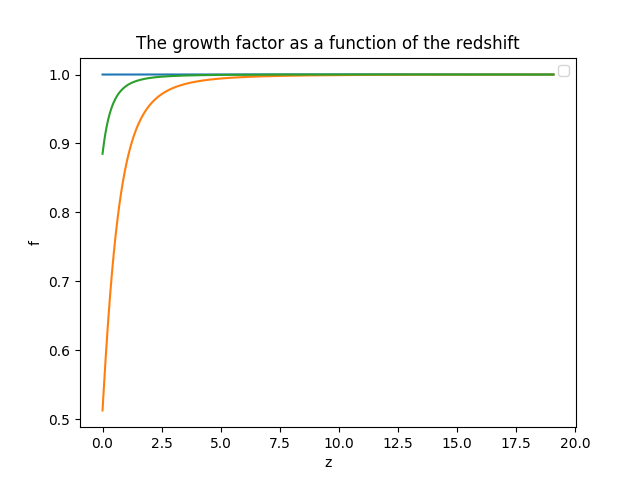
\includegraphics[scale=0.475]{exercise2-2}
\end{figure}

\noindent \textbf{Exercise 3.}\\
(1) Derive and plot the radiation and gas temperature as the universe expands, assuming it expands adiabatically:\\
\textbf{Radiation Temperature $(T_r)$:}\\
We have the equation of state for radiation pressure $p = \dfrac{u}{3} = \dfrac{\sigma T^4}{3}
$ where $\sigma$ is the Stephan-Boltzmann constant.\\
From the second law of thermodynamics we know that:

\begin{align*}
dS =& \dfrac{dU}{T} + p\dfrac{dV}{T} = 0\\
0 =& \dfrac{d(uV)}{T} + \dfrac{u}{3} \dfrac{dV}{t}\\
=& du \dfrac{V}{T} + dV \dfrac{u}{T} + \dfrac{udV}{3T}\\
=& \dfrac{4u}{3T} dV + \dfrac{V}{T} du
\end{align*}
Rearranging and using $\dfrac{du}{dT} = 4\sigma T^3$
\begin{align*}
\dfrac{4u}{3T}dV =& - \dfrac{V}{T} \dfrac{du}{dT}dT\\
\dfrac{dV}{V} =& - \dfrac{4T^3 \sigma \cdot 3T}{4 \sigma T^4 \cdot T} dT\\
=& - \dfrac{3dT}{T}
\end{align*}
And using the fact that the volue of a cube of side length $a$ is $V = a^3$, we see that $\dfrac{dV}{V} = - \dfrac{da}{a}$.\\
Therefore $T_{r} \propto a^{-1} = (1+z).$\\
\textbf{Gas Temperature $(T_m)$:}\\
We know for non-relativistic particles that $E = \dfrac{p^2}{2m}$. Utilizing the deBroglie wavelength of a particle, we can approximate the distance between particles at recombination, such that:

\begin{equation}
T \propto E \propto p^2 \propto \lambda_{dB}^{-2} \propto a^{-2} \propto (1+z)^2
\end{equation}

\begin{figure}[h]
\centering
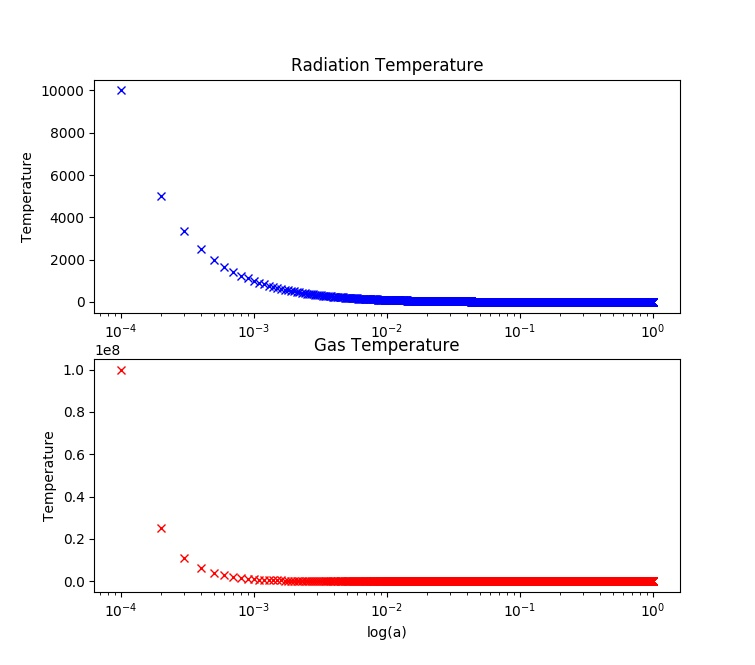
\includegraphics[scale=.35]{exercise3-1}

\end{figure}

\clearpage

\noindent\textbf{Exercise 4.}\\
Assuming an Einstein deSitter Universe [$\Omega_m = 1.0, \Omega_{\Lambda} = 0.0$] show that the parameterization

\begin{align*}
R =& A(1-\cos \theta)\\
t =& B(\theta - \sin \theta)\\
A^3 =& GMB^2
\end{align*}
\noindent satisfies $\ddot{R} = - \dfrac{GM}{R^2}$. Let's expand the L.H.S. and R.H.S. and independently to show that they are equal.\\
\begin{equation} \label{eq:12}
\ddot{R} = \dfrac{d}{d \theta} (\dfrac{dR}{dt})(\dfrac{d \theta}{dt})
\end{equation}
\noindent Solving the parts of the R.H.S. (12) independently:
\begin{align*}
\dfrac{dR}{dt} =& \dfrac{dR}{d \theta} \cdot \dfrac{d \theta}{dt} \\
\dfrac{dt}{d \theta} =& \dfrac{d}{d \theta}(B(\theta - \sin \theta)) = B(1-\cos \theta),  \dfrac{d \theta}{dt} = \dfrac{1}{\dfrac{dt}{d \theta}} = \dfrac{1}{B(1-\cos \theta)}\\ 
\dfrac{dR}{d \theta} =& \dfrac{d}{d \theta}(A(1-\cos \theta)) = A \sin \theta\\
\dfrac{dR}{dt} =& \dfrac{A \sin \theta}{B(1-\cos \theta)}
\end{align*}
Combining the terms, we see $\ddot{R}$ is equal to:\\
\begin{align}
\ddot{R} =& \dfrac{A}{B} \Big[ \dfrac{\cos \theta(1-\cos \theta) - \sin^2 \theta}{(1 - \cos \theta)^2} \Big] \cdot \dfrac{1}{B(1-\cos \theta)}\\
=& \dfrac{A}{B^2} \Big[ \dfrac{\cos - \cos^2 \theta - \sin^2 \theta}{(1-\cos \theta)^3} \Big]\\
=& \dfrac{A}{B^2} \Big[ \dfrac{\cos \theta - 1}{(1 - \cos \theta)^3} \Big]\\
=& - \dfrac{A}{B^2(1-\cos \theta)^2}
\end{align}

Now to handle the L.H.S.:
\begin{align*}
GM =& \dfrac{A^3}{B^2}\\
\dfrac{GM}{R^2} =& \Big(\dfrac{A^3}{B^2}\Big)\Big(\dfrac{1}{A(1 - \cos \theta)}\Big)^2\\
=& \dfrac{A}{B^2(1-\cos \theta)^2}
\end{align*}
So the L.H.S. is defined by:
\begin{equation}
- \dfrac{GM}{R^2} = - \dfrac{A}{B^2(1-\cos \theta)^2}
\end{equation}
And we see that $\ddot{R} = - \dfrac{A}{B^2(1-\cos \theta)^2} = -\dfrac{GM}{R^2}$
\clearpage

\noindent \textbf{Exercise 5.}\\
Derive the infall velocity $v_{infall}$ as the gas virializes. The velocity is equal to the first time derivative of the radius, so:
\begin{align*}
\dot{R} = \dfrac{dR}{dt} = \dfrac{dR}{d \theta} \cdot \dfrac{d \theta}{dt}
\end{align*}

\noindent We can use values derived in exercise 4 to show that:

\begin{equation}
\dot{R} = \dfrac{A}{B} \dfrac{\sin \theta}{(1-\cos \theta)}
\end{equation}
Virialization occurs at $ \theta = \dfrac{3 \pi}{2}$, so $\dot{R}_{vir} = - \dfrac{A}{B}$ which shows that the velocity is directed towards the center of the sphere. And $R_{vir} = A(1-0) = A.$\\
The infall velocity (towards the center) is:

\begin{equation}
v_{infall} = \dfrac{A}{B} = \sqrt{\dfrac{A^2}{B^2}} = \sqrt{\dfrac{A^3}{B^2 \cdot A}} = \sqrt{\dfrac{GM}{R_{vir}}}
\end{equation}

\noindent \textbf{Exercise 6.}\\
Show that the gravitational binding energy of a uniform sphere of radius $R$ is $U = - \dfrac{3GM^2}{5R}$.\\
Assuming uniform density $\rho$, we see $m_{shell} = 4 \pi r^2 \rho dr$ and the mass within the shell $m_{int} = \dfrac{4}{3} \pi r^3 \rho.$\\
Potential:
\begin{align*}
dU =& - \dfrac{Gm_{int}m_{shell}}{r} = - \dfrac{G(4 \pi r^2 \rho dr)(\dfrac{4}{3} \pi r^3 \rho)}{r}\\
=& - G \dfrac{16}{3} \pi^2 r^4 \rho^2 dr
\end{align*}
Integrating over the whole sphere, radially:
\begin{equation}
U = -G \int_0^R \dfrac{16}{3} \pi^2 r^4 \rho^2 dr = -G \dfrac{16}{3} \pi^2 \rho^2 \int_0^R r^4 dr = -G \dfrac{16}{15} \pi^2 \rho^2 R^5
\end{equation}
Reintroducing $\rho = \dfrac{M}{\dfrac{4}{3} \pi R^3},$ equation (17) becomes:
\begin{equation}
U = - G \dfrac{16}{15} \pi^2 \dfrac{M^2}{\dfrac{16}{9}\pi^2 R^6}R^5 = - \dfrac{9}{15} \dfrac{GM^2}{R} = - \dfrac{3}{5} \dfrac{GM^2}{R}
\end{equation}

\end{document}